%!TEX encoding = UTF-8 Unicode

\documentclass[12pt, a4paper]{article}

\usepackage{color}
\usepackage{url}
\usepackage[T2A]{fontenc} 
\usepackage[utf8]{inputenc} 
\usepackage{graphicx}
\usepackage{hyperref}
% \usepackage[
% backend=biber,
% style=numeric,
% sorting=none
% ]{biblatex}
\usepackage{biblatex}
\hypersetup{
    colorlinks=true,
    linkcolor=blue,
    filecolor=magenta,      
    urlcolor=blue,
}



\usepackage[english,serbian]{babel}

% \usepackage[unicode]{hyperref}
% \hypersetup{colorlinks,citecolor=green,filecolor=green,linkcolor=blue,urlcolor=blue}


\begin{document}

\title{Privatni nalozi na društvenim mrežama\\Neophodnost ili ne?\\ \small{Kurs: Računarstvo i društvo\\ Matematički fakultet}}

\author{Anđela Niketić}
\date{\today}
\maketitle

\abstract{
Društveni mreže su interaktivne računarski posredovane tehnologije koje olakšavaju stvaranje ili razmenu informacija, ideja, interesa u karijeri i drugih oblika izražavanja putem virtuelnih zajednica i mreža. One služe za međusobno povezivanje korisinka i postale su neizostavan
deo svakodnevnog života za milijarde ljudi širom sveta.

\tableofcontents

\newpage

\section{Uvod}

Društvene mreže predstavljaju ključni fenomen savremenog digitalnog doba, transformišući način na koji ljudi komuniciraju, povezuju se i dele informacije. Sa ekspanzijom interneta i razvojem tehnologije, društvene mreže postale su centralno mesto za interakciju, stvaranje zajednica i izražavanje identiteta u onlajn prostoru. Bez obzira da li se radi o popularnim platformama poput Facebook-a, X-a (Twitter-a), Instagram-a ili novijim mrežama specijalizovanim za određene interese, društvene mreže obuhvataju širok spektar funkcija i mogućnosti koje omogućavaju korisnicima da se povežu sa prijateljima, porodicom, kolegama i širom globalnom zajednicom. 


Kroz svoje različite oblike, društvene mreže postale su neizostavan deo svakodnevnog života milijardi ljudi širom sveta, pružajući prostor za izražavanje, informisanje, zabavu i aktivizam. U ovom kontekstu, razumevanje fenomena društvenih mreža postaje ključno za sagledavanje modernog digitalnog društva i njegovih dinamičnih interakcija.


Međutim, sa porastom zabrinutosti za privatnost i bezbednost na internetu, sve veći broj korisnika okreće se ka privatnim nalozima na društvenim mrežama. U ovom esejnom radu istražićemo kako se privatni profili uklapaju u širi kontekst društvenih mreža, analizirajući njihovu svrhu, uticaj i implikacije za korisnike i društvo u celini. Kroz ovu analizu, pokušaćemo da bolje razumemo dinamiku između privatnosti, kontrole i društvenog angažovanja u digitalnom okruženju društvenih mreža.


\newpage


\section{Privatnost i bezbednost na internetu}	
\label{sec:sigurnost}

Deljenje privatnih informacija putem društvenih medija je uobičajeno u današnjem društvu i načinu života. Korisnici dele svoje privatne informacije, posebno prilikom registracije kako bi uopšte postali članovi društvenih mreža, ne uzimajući u obzir da se te informacije mogu zloupotrebiti. Takođe, otkrivaju svoje privatne informacije putem redovnih ažuriranja i objava koje postavljaju na mreži. Kao rezultat toga, pojedincu se može lako ući u trag i manipulisati putem informacija koje dele na ovim veb lokacijama, što čini internet privatnost glavnim problemom.


Jedan od nedostataka društvenih medja je izlaganje privatnog života ljudi širom interneta, pa time i širom sveta. Danas je pitanje deljenja previše ličnih informacija postalo društveni standard, zaboravljajući da se te informacije mogu koristiti na različite načine, uključujući i uhođenje pa čak i krađu identiteta. Korisnici društvenih mreža moraju da preispitaju informacije koje dele na internetu kao i sa kim ih dele.
Temeljna svest o pitanjima privatnosti na društvenim mrežama je od suštinskog značaja kako bi se korisnici ogradili i izbegli zloupotrebu informacija na internetu.

Na osnovu istraživanja \textbf{Pew Research centra} iz 2022. godine\cite{pew2022}, čak \textbf{95\%} ispitanika (uzrasta od 13 do 17 godina) izjavilo je da  koriste društvene mreže, a više od trećine izjavljuje da ih koristi „skoro konstantno“. Isto istraživanje, pokazalo je i da 6 od 10 tinejdžera smatraju da imaju malo \textbf{(40\%) }do nikakvu kontrolu \textbf{(20\%)} nad ličnim podacima koje društvene mreže prikuljaju o njima. Dodatnih \textbf{26\%  }čak nisu ni sigurni koliku kontrolu nad podacima uopšte imaju. Samo \textbf{14\%} tinejdžera smatra da ima veliku kontrolu nad svojim podacima.

\begin{figure}[h]
    \centering
    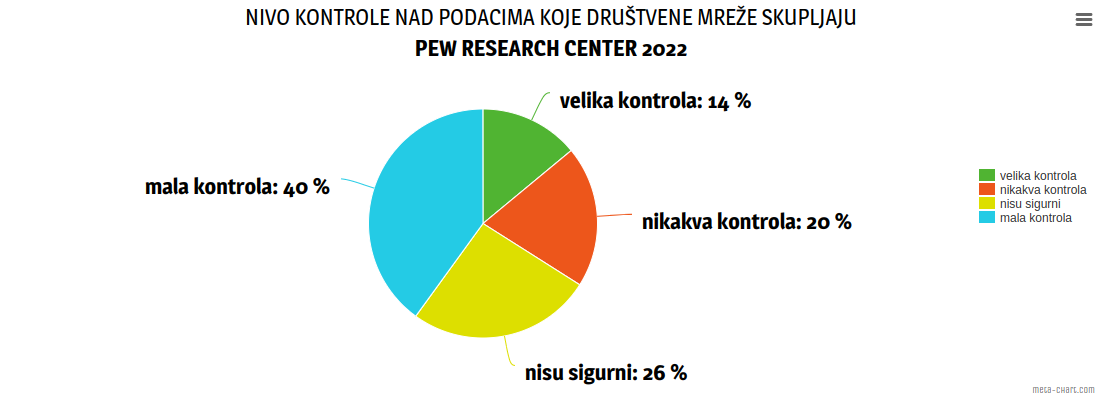
\includegraphics[scale = 0.3]{stats.png}
    \label{fig:graf1}
    \caption{Nivo kontrole nad podacima}
\end{figure}

\newpage
\section{Privatni profili}
\subsection{Šta su privatni i javni profili?}
\label{sec:Priv}

\textbf{Privatni profili }na društvenim mrežama predstavljaju korisničke naloge koji ograničavaju vidljivost i dostupnost sadržaja samo na određene korisnike ili grupu korisnika. Ovi profili omogućavaju korisnicima da kontrolišu ko može da pristupi njihovom profilu i sadržaju koji dele, što može obuhvatiti fotografije, objave, lične informacije i druge podatke. 


Za razliku od \textbf{javnih profila} koji su dostupni i vidljivi svima na internetu, privatni profili zahtevaju od korisnika određene radnje kako bi pristupili korisničkom sadržaju, kao što su zahtevi za prijateljstvo, odobrenje pratilaca ili upotreba lozinki za pristup. Kroz korišćenje privatnih profila, korisnici mogu bolje kontrolisati svoju online prisutnost, štiteći privatnost svojih podataka i ograničavajući pristup svojim informacijama samo na odabrane osobe ili grupe. Ovi profili često pružaju osećaj sigurnosti i intimnosti korisnicima, omogućavajući im da se slobodnije izraze i komuniciraju unutar zaštićenog okruženja.

\subsection{Koliko ljudi koristi privatne profile?}

Istraživanja pokazuju da ljudi sve češće preduzimaju korake da ograniče pristup svojim privatnim informacijama. Više od polovine korisnika ima privatne profile na društvenim mrežama, od čega su većinski žene, što dalje ukazuje na to da su one više zabrinute za svoju privatnost u odnosu na muškarce.


Uzimajući u obzir da su najaktivniji korisnici društvenih mreža mladi ljudi, većina istraživanja se fokusira upravo na njih. Na osnovu istraživanja \textit{\textbf{Pew Research centra}} iz 2012. godine \cite{pew2012}, oko \textbf{60\%} ispitanih tinejdžera (uzrasta od 12 do 17 godina) koji koriste Facebook, kažu da je njihov profil podešen na \textbf{privatan} tako da samo njihovi prijatelji mogu da ga vide. S druge strane, \textbf{25\%} izjavljuje da ima \textbf{delimično privatan} profil tako da prijatelji njihovih prijatelja mogu da vide šta objavljuju. Dok \textbf{14\%} tinejdžera kaže da je njihov profil \textbf{potpuno javan}.

S druge strane, korisnici \textbf{Twitter-a} većinski biraju javne profile - 64\% tinejdžera. Zabrinjavajuća statistika iz ovog istraživanja je ta da čak 12\% tinejdžera ne znaju da li im je Twitter profil javan ili privatan.


% \begin{figure}[h!]
%     \centering
%     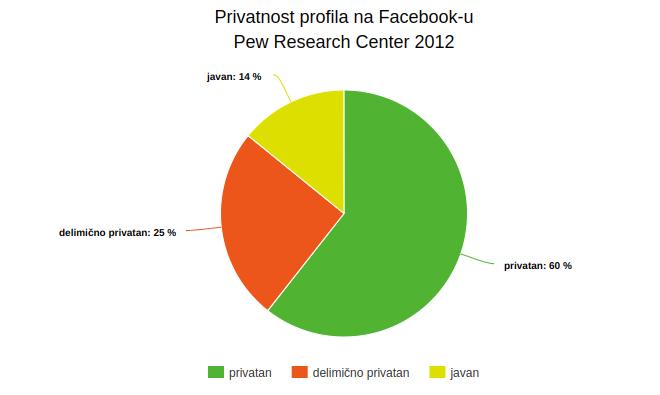
\includegraphics[scale = 0.6]{graf2.png}
%     \label{fig:graf2}
%     \caption{Privatnost profila na Facebook-u}
% \end{figure}

% \begin{figure}[h!]
%     \centering
%     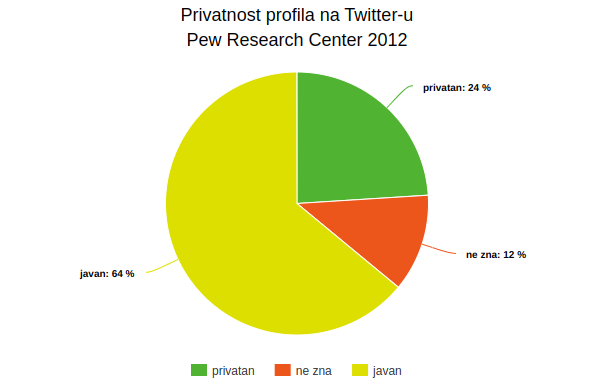
\includegraphics[scale = 0.6]{graf3.png}
%     \label{fig:graf3}
%     \caption{Privatnost profila na Twitter-u}
% \end{figure}


\begin{figure}
\centering
\begin{minipage}{.5\textwidth}
  \centering
  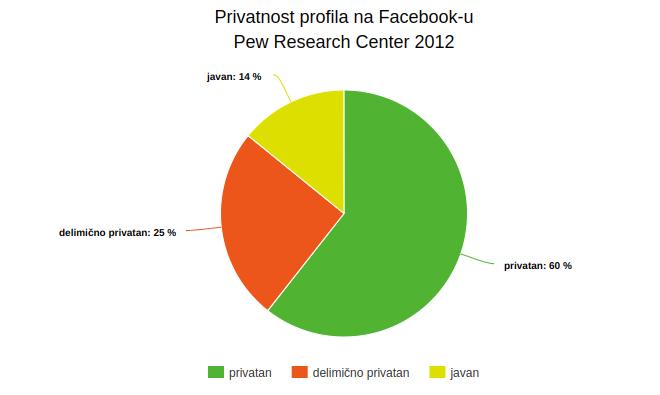
\includegraphics[width = 8cm]{graf2.png}
  \label{fig:test1}
\end{minipage}%
\begin{minipage}{.5\textwidth}
  \centering
  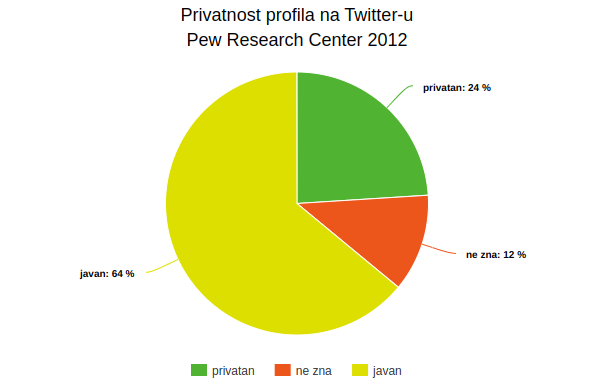
\includegraphics[width=8cm]{graf3.png}
  \label{fig:test2}
\end{minipage}

  \caption{Privatnost profila na Facebook-u i Twitter-u}
\end{figure}


\newpage

\section{Prednosti i mane privatnih profila}
U prethodnim sekcijama, objasnili smo šta su privatni profili, kakve funkcije nam pružaju i koliko korisnika zapravo koristi ovu opciju. U ovom odeljku, detaljnije ćemo obraditi prednosti i mane imanja privatnog profila na društvenim mrežama.

Jedan od glavnih razloga za korišćenje privatnih profila je \textbf{očuvanje privatnosti}. 
Smanjujemo rizik od zloupotrebe naših podataka, fotografija, izjava, time što \textit{zaključamo} naš profil. 
Ovim putem, samo korisnici kojima mi dozvolimo pristup mogu da vide naše objave, ali da li smo onda u potpunosti sigurni da baš ti korisnici neće zloupotrebiti ovu privilegiju? Svodi se na poverenje, potrebno nam je poverenje kako bismo delili objave, ali što više delimo, imamo manje privatnosti. Odnos je paradoksalan.
Skoro sve što radimo na društvenim mrežama se svodi na \textbf{poverenje}. Da li verujemo da će platforma zaštititi naše podatke? Verujemo li svemu što vidimo i pročitamo na internetu? Da li verujemo korisnicima koji vide naše objave?
Prema istraživanjima \cite{cyberology}, korisnici privatnih profila generalno imaju viši nivo poverenja od korisnika javnih profila.

Popularan razlog za odabir privanog profila je \textbf{povezivanje sa bliskim ljudima}. Neki korisnici jednostavno žele da budu u kontaktu, i dele objave samo sa bliskim prijateljima i porodicom. Veruju da ovim pristupom ojačavaju odnose sa najbližima. Sama sloboda izbora ko će nas pratiti daje samopouzdanje i poverenje. Izbegavaju se neželjene interakcije, poruke, lažni nalozi...

Privatni nalozi ne garantuju sigurnost i poverljivost na internetu. Deljenje previše privatnih informacija može dovesti do neželjenih situacija. Iako privatni nalozi pružaju dosta načina za kontrolu protoka informacija, ne garantuju sigurnost na internetu. Čak i pri odabiru privatnih naloga, delimo neki deo naših informacija.
Na Instagram profilima, iako su privatni, svima su vidljive informacije poput imena i kratke biografije kao i profilne slike. Ovako mala količina informacija može biti dovoljna zlonamernim posmatračima.


\begin{figure}[h!]
     \centering
     
\includegraphics[scale = 0.6]{priv.png}
     \label{fig:privatni profil}
     \caption{Izgled privatnog profila na Instagramu}
 \end{figure}

Našim informacijama ne pristupaju samo drugi korisnici, već i sama društvena mreža koju koristimo. Društvene mreže prate naše \textbf{interakcije} kako bi nam preporučile što bolji sadržaj sa kojim bismo dalje interagovali, sve u cilju da nam povećaju vreme koje provodimo na toj platformi. Što više interagujemo, to se više informacija skuplja i više sadržaja nam se preporučuje. 
Ove informacije ne možemo kontrolisati u meri koju bismo voleli, možemo smanjiti \textit{screen time}, smanjiti interakcije, izbegavati društvene mreže celokupno, ali već smo naviknuti da konzumiramo sadržaj i interagujemo sa ljudima preko društvenih mreža jer su postale neizostavan deo svakodnevnog života.





\section{Zaključak}
\label{sec:zakljucak}

Na početku, društvene mreže su bile isključivo korišćene za komunikaciju, a sada su postale sastavni deo naših života. Ključno je pronaći balans između privatnosti i vidljivosti na internetu, i doneti informisanu odluku o tome kakav profil želimo da koristimo.


\addcontentsline{toc}{section}{Literatura}
\appendix

\medskip 

\begin{thebibliography}{9}
    \bibitem[1]{pew2022} \href{https://www.pewresearch.org/short-reads/2023/04/24/teens-and-social-media-key-findings-from-pew-research-center-surveys/}{ Teens and social media: Key findings from Pew Research Center surveys, 2022}
    
    \bibitem[2]{pew2012} \href{https://www.pewresearch.org/short-reads/2023/04/24/teens-and-social-media-key-findings-from-pew-research-center-surveys/}{Teens, Social Media, and Privacy, 2012 }
    
    \bibitem[3]{cyberology} 
    \href{https://www.cybercology.com/2020/09/17/who-is-more-trusting-people-with-a-private-or-public-profile/}{Who is more trusting? People with a private or public profile? 2020, Carolyn Freeman}

    \bibitem[4]{guillem}  \href{https://guillemrecolons.com/en/ventajas-perfiles-privados/#:~:text=The%20researchers%20found%20that%20people,less%20exposure%20to%20unwanted%20contact.}{Advantages and disadvantages of private profiles on social networks, 2023, Guillem Recolons}
\end{thebibliography}



\appendix



\end{document}
